\section{Варианты использования}
Все варианты использования, определенные в системе, приведены на рисунке~\ref{fig:useCases}.
	\subsection{Диаграмма вариантов использования}
		\begin{figure}[h]
			\center{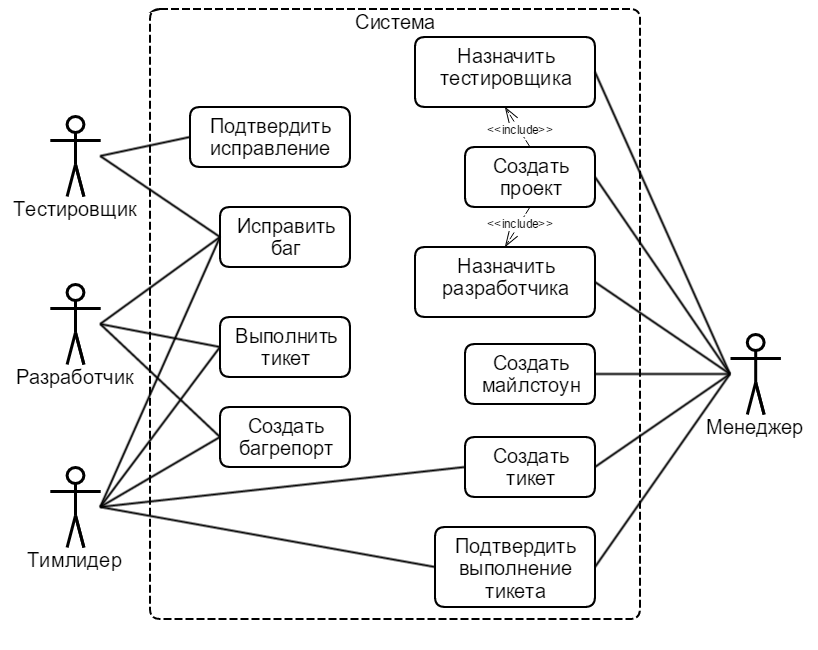
\includegraphics[width=\linewidth]{useCases}}
			\caption{Варианты использования}
			\label{fig:useCases}
		\end{figure}
	
	\subsection{Описание вариантов использования}
		\subsubsection{Запись пациента на прием}
			Разработка проекта:
			\begin{itemize}
				\item менеджер создает новый проект;
				\item менеджер добавляет разработчиков в проект;
				\item менеджер добавляет тестировщиков в проект;
				\item менеджер определяет тимлидера;
				\item менеджер определяет майлстоуны проекта и назначает даты;
				\item менеджер выдает тикеты разработчикам;
				\item разработчики выполняют тикеты ближайшего майлстоуна;
				\item предыдущие три шага итеративно повторяются до завершения проекта;
				\item проект завершается.
			\end{itemize}
			
			Выполнение тикета:
			\begin{itemize}
				\item менеджер/тимлидер создает новый тикет;
				\item менеджер/тимлидер определяет разработчиков-исполнителей. Тикет получает статус "новый";
				\item разработчик получает уведомление о новом тикете и меняет его статус на "принят";
				\item разработчик приступает к выполнению задания. Тикет получает статус "в процессе выполнения";
				\item разработчик выполняет задание и меняет статус тикета на "выполнен";
				\item менеджер/тимлидер проверяет и подтверждает выполнение задания. Тикет получает задание "закрыт".
			\end{itemize}
			
			Обработка ошибки:
			\begin{itemize}
				\item разработчик/тестировщик создает отчет с описанием ошибки. Отчет получает статус "новый";
				\item разработчик принимает уведомление и меняет статус отчета на "активен";
				\item разработчик исправляет баг и меняет статус на "исправлен";
				\item тестировщик проверяет исправление и закрывает отчета указав ему статус "закрыт".
			\end{itemize}